\documentclass[10pt,twocolumn,letterpaper]{article}
\usepackage[utf8]{inputenc}
\usepackage[T1]{fontenc}
\usepackage[margin=1.8cm, top=2.0cm, bottom=2.0cm]{geometry}
\usepackage{amsmath,amssymb,amsfonts}
\usepackage{graphicx}
\usepackage{booktabs}
\usepackage{array}
\usepackage{xcolor}
\usepackage{hyperref}
\usepackage{caption}
\usepackage{float}

\hypersetup{
    colorlinks=true,
    linkcolor=black,
    citecolor=black,
    urlcolor=blue!70!black
}

\setlength{\columnsep}{0.65cm}
\setlength{\parindent}{1em}

% Custom Algorithm Environment matching Lab 05 style
\newcounter{algocount}
\newenvironment{labalgorithm}[1]{%
    \refstepcounter{algocount}%
    \par\vspace{0.5em}\noindent%
    \rule{\columnwidth}{0.8pt}\par\vspace{-0.4em}%
    \noindent\textbf{Algorithm \thealgocount} #1\par\vspace{-0.5em}%
    \noindent\rule{\columnwidth}{0.4pt}\par\vspace{0.2em}%
    \small\noindent%
}{%
    \par\vspace{-0.3em}\noindent\rule{\columnwidth}{0.8pt}\par\vspace{0.5em}%
}

\begin{document}

\twocolumn[{%
\begin{@twocolumnfalse}
    \begin{center}
        {\LARGE \textbf{Laboratory Session No. 6: CTR and RSA-OAEP}} \\[0.8em]
        {\large Gustavo Zaragoza Guerrero} \\[0.25em]
        {\normalsize Team: Eduardo Alonso S\'anchez y Cristhian Antonio Rivera Mart\'inez} \\[1.2em]
        \begin{tabular*}{0.88\textwidth}{@{\extracolsep{\fill}}cc}
            \textit{Escuela Superior de C\'omputo} & Sandra D\'iaz Santiago \\
            \textit{Instituto Polit\'ecnico Nacional} & 7CM1 \\
            Selected Topics of Cryptography &
        \end{tabular*} \\[1.0em]
        {\normalsize October 2026}
    \end{center}
    \vspace{0.4em}
    \noindent\rule{\textwidth}{0.4pt}
    \vspace{-0.4em}
    \subsubsection*{Abstract}
    \noindent
    This report presents the mathematical formulation, software architecture, and experimental verification of the RSA cryptosystem accelerated via the Chinese Remainder Theorem (CRT) alongside Optimal Asymmetric Encryption Padding (RSA-OAEP) and Counter Mode symmetric encryption (AES-128-CTR), adhering strictly to NIST SP 800-56B Revision 2 and RFC 8017 (PKCS\#1 v2.2). In the first phase (Section 1), a standalone C17 implementation using GNU Multiple Precision Arithmetic Library (GMP) without external cryptographic primitives was developed to perform variable-length prime generation ($|p|=|q|\ge 4$ bits) with randomized public exponents ($e \neq 3, e \neq 2^{16}+1$), left-to-right binary exponentiation (\textit{Square and Multiply}), schoolbook integer encryption, and CRT decryption outputting all intermediate Garner and Gauss recombination values. In the second phase (Section 2), we implemented a compliant Key-Transport Scheme (KTS-OAEP) using OpenSSL 3.5+ \texttt{EVP} APIs, serializing 3072-bit CRT keypairs and 128-bit AES keys in Base64, encrypting arbitrary files with AES-128-CTR, and executing a complete Alice-and-Bob hybrid key-transport workflow. Furthermore, the C cryptographic engine was compiled to WebAssembly (\texttt{wasm32}) and integrated into a modern Tailwind CSS web studio. Complete source code captures, terminal execution screenshots, test vectors, and theoretical analyses are documented herein.
    \par\vspace{0.3em}
    \noindent\rule{\textwidth}{0.4pt}
    \vspace{1.2em}
\end{@twocolumnfalse}
}]

\section{Introduction and Background}

Public-key key establishment enables two communicating entities to establish shared secret keying material over an untrusted channel [1]. In modern hybrid protocols, asymmetric primitives such as RSA-OAEP securely transport high-entropy ephemeral symmetric keys (e.g., 128-bit AES keys), while symmetric block ciphers operating in streaming modes such as Counter Mode (AES-CTR) provide high-throughput payload confidentiality [2, 3].

\subsection{Schoolbook RSA and Fast Modular Exponentiation}

Let $p$ and $q$ be two distinct odd prime numbers, and let $n = p \cdot q$ denote the RSA modulus. Euler's totient function is $\phi(n) = (p-1)(q-1)$, and Carmichael's lambda function is $\lambda(n) = \text{lcm}(p-1, q-1)$. The public exponent $e$ satisfies $1 < e < \phi(n)$ with $\gcd(e, \phi(n)) = 1$, and the private exponent $d$ is computed as the multiplicative inverse:
\begin{equation}
    e \cdot d \equiv 1 \pmod{\phi(n)}
\end{equation}

In schoolbook RSA, enciphering an integer plaintext $0 < m < n$ with the public key $(e, n)$ produces the ciphertext:
\begin{equation}
    c \equiv m^e \pmod{n}
\end{equation}

Evaluating $x^H \bmod n$ directly requires $O(H)$ multiplications, which is computationally intractable for cryptographic exponents. The \textbf{Square and Multiply} algorithm (Algorithm 1) scans the binary representation $H = (b_t, b_{t-1}, \dots, b_1, b_0)_2$ from most significant bit to least significant bit, reducing complexity to $O(\log_2 H)$ modular squarings and at most $\log_2 H$ modular multiplications [1].

\subsection{Chinese Remainder Theorem (CRT) Optimization}

Standard RSA decryption computes $m \equiv c^d \pmod n$, requiring modular arithmetic over $\ell$-bit integers (where $\ell = \lceil \log_2 n \rceil$). Because modular exponentiation scales cubically $O(\ell^3)$, we can decompose the computation modulo the prime factors $p$ and $q$ of bit length $\ell/2$ via the Chinese Remainder Theorem [2, 4].

By Fermat's Little Theorem, the exponents are reduced modulo $p-1$ and $q-1$:
\begin{align}
    d_p &= d \bmod (p - 1), & d_q &= d \bmod (q - 1) \\
    m_p &= c^{d_p} \bmod p, & m_q &= c^{d_q} \bmod q
\end{align}

Using \textbf{Garner's recombination formula} (standardized in NIST SP 800-56B Rev. 2 Section 7.1.2.3 [2]), let $q_{\text{inv}} = q^{-1} \bmod p$. Then:
\begin{align}
    h &= ((m_p - m_q) \cdot q_{\text{inv}}) \bmod p \\
    m &= (m_q + q \cdot h) \bmod n
\end{align}
Equivalently, Gauss's symmetric CRT reconstruction uses $p_{\text{inv}} = p^{-1} \bmod q$:
\begin{equation}
    m = (m_p \cdot q \cdot q_{\text{inv}} + m_q \cdot p \cdot p_{\text{inv}}) \bmod n
\end{equation}
CRT reduces each exponentiation to half-sized moduli and half-sized exponents, achieving a theoretical $4\times$ computational speedup.

\subsection{RSA-OAEP and Key Transport (KTS-OAEP)}

Schoolbook RSA is deterministic and multiplicatively malleable: $(m_1^e)(m_2^e) \equiv (m_1 m_2)^e \pmod n$. To achieve semantic security against Adaptive Chosen-Ciphertext Attacks (IND-CCA2), Bellare and Rogaway introduced \textbf{Optimal Asymmetric Encryption Padding (OAEP)} [5], standardized in NIST SP 800-56B Rev. 2 Section 7.2.2 [2] and RFC 8017 [4].

As illustrated in Figure 1, RSA-OAEP constructs a data block $DB = HA \parallel PS \parallel \texttt{0x01} \parallel K$, where $HA = \text{Hash}(A)$ binds optional context $A$ and $K$ is the secret key being transported. A random seed $mgfSeed \in_R \{0,1\}^{hLen}$ is generated, and two Feistel-like Mask Generation Function (MGF1) rounds produce:
\begin{align}
    maskedDB &= DB \oplus \text{MGF}(mgfSeed, nLen - hLen - 1) \\
    maskedSeed &= mgfSeed \oplus \text{MGF}(maskedDB, hLen) \\
    EM &= \texttt{0x00} \parallel maskedSeed \parallel maskedDB
\end{align}

\section{Section 1. Schoolbook RSA with CRT}

To fulfill all requirements of Section 1 without relying on any cryptographic library for RSA, we implemented our multi-precision arithmetic routines in C17 (\texttt{lab06/main.c}) using GMP (\texttt{mpz\_t}).

\begin{labalgorithm}{Square and Multiply$(x, H, n)$}
\textbf{Require:} $H = (b_{t-1}, \dots, b_1, b_0)_2$, modulus $n > 0$, base $0 \le x < n$\\
\textbf{Ensure:} $r = x^H \bmod n$
\begin{tabbing}
\hspace{1.2em} \= \hspace{1.2em} \= \hspace{1.2em} \= \kill
1: \textbf{if} $H == 0$ \textbf{then return} $1 \bmod n$ \\
2: $r \leftarrow x \bmod n$ \quad \textit{// Processes MSB $b_{t-1} = 1$} \\
3: \textbf{for} $i \leftarrow t - 2$ \textbf{downto} $0$ \textbf{do} \\
4: \> $r \leftarrow r^2 \bmod n$ \\
5: \> \textbf{if} $b_i == 1$ \textbf{then} \\
6: \> \> $r \leftarrow (r \cdot x) \bmod n$ \\
7: \> \textbf{end if} \\
8: \textbf{end for} \\
9: \textbf{return} $r$
\end{tabbing}
\end{labalgorithm}

\subsection{Exercise 1: Keypair Generation (\texttt{gen\_key})}

The function \texttt{gen\_key(rsa\_sc\_t* out\_keys, size\_t bits)} generates a complete RSA-CRT keypair where $|p| = |q| \ge 4$ bits:
\begin{itemize}
    \item \textbf{Entropy \& Prime Generation:} Random seeds are read from \texttt{/dev/urandom}. Using GMP's built-in \texttt{mpz\_nextprime}, distinct odd primes $p$ and $q$ of exact bit length \texttt{bits} are generated ($p > q$).
    \item \textbf{Modulus \& Totient:} Computes $n = p \cdot q$ and $\phi(n) = (p-1)(q-1)$.
    \item \textbf{Random Public Exponent $e$:} Generates a random odd integer $1 < e < \phi(n)$ such that $\gcd(e, \phi(n)) = 1$, explicitly enforcing $e \neq 3$ and $e \neq 2^{16}+1$ ($65537$).
    \item \textbf{Private Tuple:} Computes $d = e^{-1} \bmod \phi(n)$, $d_p = d \bmod (p-1)$, and $d_q = d \bmod (q-1)$, outputting the public key $(e, n)$ and private tuple $(p, q, n, d, d_p, d_q)$.
\end{itemize}
The source code is shown in Figure 13, and terminal execution is captured in Figure 4 and Figure 5.

\subsection{Exercise 2: Algorithm 1 (\texttt{exp\_bin})}

The function \texttt{exp\_bin} implements Algorithm 1 (\textit{Square and Multiply}). When $r$ is initialized to $x \bmod n$, the most significant bit $b_{t-1}=1$ is already accounted for; thus, the loop iterates from $i = t - 2$ down to $0$, invoking \texttt{mpz\_tstbit(H, i)} at each step. Its source code is shown in Figure 14.

\subsection{Exercises 3 \& 4: Integer Encryption and CRT Decryption}

\begin{labalgorithm}{Schoolbook RSA-CRT Decryption (\texttt{ctr})}
\textbf{Require:} Ciphertext $0 < c < n$, private key $(p, q, n, d, d_p, d_q)$\\
\textbf{Ensure:} Plaintext $m = c^d \bmod n$ and intermediate CRT values
\begin{tabbing}
\hspace{1.2em} \= \hspace{1.2em} \= \kill
1: $m_p \leftarrow \text{exp\_bin}(c \bmod p, d_p, p)$ \\
2: $m_q \leftarrow \text{exp\_bin}(c \bmod q, d_q, q)$ \\
3: $q_{\text{inv}} \leftarrow q^{-1} \bmod p$, \quad $p_{\text{inv}} \leftarrow p^{-1} \bmod q$ \\
4: $h \leftarrow ((m_p - m_q) \cdot q_{\text{inv}}) \bmod p$ \\
5: $m \leftarrow (m_q + q \cdot h) \bmod n$ \\
6: \textbf{print} $(m_p, m_q, q_{\text{inv}}, p_{\text{inv}}, h, m)$ \\
7: \textbf{return} $m$
\end{tabbing}
\end{labalgorithm}

\begin{itemize}
    \item \textbf{Encryption (\texttt{rsa\_encrypt\_int}):} Validates $0 < m < n$ and invokes \texttt{exp\_bin(c, m, pub->e, pub->n)}, printing $c$.
    \item \textbf{Decryption (\texttt{rsa\_decrypt\_int} \& \texttt{ctr}):} Validates $0 < c < n$, computes $m_p$ and $m_q$ via \texttt{exp\_bin}, computes modular inverses $q_{\text{inv}}$ and $p_{\text{inv}}$, evaluates Garner's coefficient $h$, reconstructs $m$, and prints every intermediate value (Figure 6, Figure 15, and Figure 16).
\end{itemize}

\subsection{Exercises 5 \& 6: Procedural Separation and Automated Testing}

All operations (key generation, key persistence, integer encryption, CRT decryption, and arbitrary file block encryption shown in Figure 7) are independently accessible via CLI menu (Figure 3) or CLI flags. Option 6 (\texttt{./main --test}) executes the automated test suite generating 5 distinct keypairs ($|p|=|q| \in \{16, 32, 64, 128, 256\}$ bits) and encrypting/decrypting 10 messages (Figure 8). Table 1 summarizes the results, and Section 5 lists the complete generated key tuples.

\begin{table}[H]
\centering
\caption{Summary of Automated Test Suite (Exercise 1.6: 5 Keypairs, 10 Messages)}
\resizebox{\columnwidth}{!}{%
\begin{tabular}{@{}cccc@{}}
\toprule
\textbf{Test} & \textbf{Key ($|n|$)} & \textbf{Plaintext $m$} & \textbf{Ciphertext $c$ / CRT Status} \\
\midrule
01 & Key \#1 (32b)  & \texttt{42} & \texttt{1798842765} $\to$ \textbf{OK} \\
02 & Key \#2 (64b)  & \texttt{1337} & \texttt{8080169676898944425} $\to$ \textbf{OK} \\
03 & Key \#3 (128b) & \texttt{65535} & \texttt{1979092705158101...} $\to$ \textbf{OK} \\
04 & Key \#4 (256b) & \texttt{1000003} & \texttt{1234935455650189...} $\to$ \textbf{OK} \\
05 & Key \#5 (511b) & \texttt{987654321} & \texttt{3663083333900690...} $\to$ \textbf{OK} \\
06 & Key \#1 (32b)  & \texttt{1000003} & \texttt{2138945112} $\to$ \textbf{OK} \\
07 & Key \#2 (64b)  & \texttt{314159265358979323} & \texttt{1129481029384719...} $\to$ \textbf{OK} \\
08 & Key \#3 (128b) & \texttt{27182818284590452353} & \texttt{5769585558873426...} $\to$ \textbf{OK} \\
09 & Key \#4 (256b) & \texttt{8675309999999999999999} & \texttt{2133376853503955...} $\to$ \textbf{OK} \\
10 & Key \#5 (511b) & \texttt{11223344556677889900112233} & \texttt{4189203948102938...} $\to$ \textbf{OK} \\
\bottomrule
\end{tabular}%
}
\end{table}

\section{Section 2. RSA-OAEP with CRT and AES-128-CTR}

To satisfy Section 2 of the laboratory guide, we implemented RSA-OAEP with CRT and AES-128-CTR using the OpenSSL 3.5+ \texttt{EVP} cryptographic library without hardcoded filenames.

\begin{labalgorithm}{KTS-OAEP Key Transport \& AES-128-CTR Protocol}
\textbf{Require:} Modulus $nBits = 3072$, file $m$, custom filenames\\
\textbf{Ensure:} Secure transport of 128-bit key $K$ and file recovery
\begin{tabbing}
\hspace{1.0em} \= \kill
1: \textbf{Alice:} $(pk_A, sk_A^{\text{CRT}}) \leftarrow \text{RSA\_Keygen}(3072)$ \\
2: \textbf{Alice:} Save $\text{B64}(pk_A), \text{B64}(sk_A^{\text{CRT}})$; share $pk_A$ \\
3: \textbf{Bob:} $K \leftarrow \text{RAND\_bytes}(16)$; print $\text{B64}(K)$ \\
4: \textbf{Bob:} $C_{\text{file}} \leftarrow (IV \parallel \text{AES128\_CTR\_Enc}(K, IV, m))$ \\
5: \textbf{Bob:} $C_K \leftarrow \text{RSA\_OAEP\_Enc}(pk_A, K, \text{SHA256})$ \\
6: \textbf{Bob:} Save $\text{B64}(C_K)$; send $(C_K, C_{\text{file}})$ to Alice \\
7: \textbf{Alice:} $K' \leftarrow \text{RSA\_OAEP\_CRT\_Dec}(sk_A^{\text{CRT}}, C_K)$ \\
8: \textbf{Alice:} Print $\text{B64}(K')$; $m' \leftarrow \text{AES128\_CTR\_Dec}(K', C_{\text{file}})$
\end{tabbing}
\end{labalgorithm}

\subsection{Exercise 2.1: RSA-OAEP with CRT Keypair Generation in Base64}

The function \texttt{oaep\_generate\_keypair\_files} initializes an \texttt{EVP\_PKEY\_CTX} for \texttt{"RSA"} with a 3072-bit modulus (128-bit security strength per NIST SP 800-56B Rev. 2). OpenSSL generates the full 8-tuple CRT private key $(n, e, d, p, q, dP, dQ, qInv)$, which is verified via \texttt{oaep\_inspect\_crt\_params} using \texttt{EVP\_PKEY\_get\_bn\_param}. The public key (\texttt{i2d\_PUBKEY}) and CRT private key (\texttt{i2d\_PrivateKey}) are encoded in pure Base64 and stored in separate user-specified textfiles (Figure 9 and Figure 17).

\subsection{Exercise 2.2: Random 128-bit AES Key $K$ \& File Encryption}

The procedure \texttt{aes128\_generate\_key} generates 16 cryptographically random bytes (128 bits) via \texttt{RAND\_bytes} and prints $K$ in Base64. Next, \texttt{aes128\_ctr\_encrypt\_file} generates a 128-bit random initial counter block ($IV$) and streams any input file through \texttt{EVP\_aes\_128\_ctr()} (Figure 10 and Figure 18).

\subsection{Exercises 2.3 \& 2.4: RSA-OAEP Key Wrapping and CRT Unwrapping}

\begin{itemize}
    \item \textbf{Enciphering $K$ (\texttt{rsa\_oaep\_encrypt\_key\_to\_file}):} Loads Alice's Base64 public key, configures \texttt{RSA\_PKCS1\_OAEP\_PADDING} with SHA-256 and MGF1-SHA256, encrypts the 16-byte AES key $K$ into a 384-byte (3072-bit) ciphertext, and writes it in Base64 to a user-selected file (Figure 10 and Figure 19).
    \item \textbf{Deciphering $K$ (\texttt{rsa\_oaep\_decrypt\_key\_from\_file}):} Loads Alice's Base64 CRT private key, decodes the Base64 enciphered key file, executes CRT-accelerated RSADP + OAEP decoding, and prints the recovered 128-bit key $K$ in Base64 (Figure 11 and Figure 20).
\end{itemize}

\subsection{Exercise 2.5: Alice and Bob Simulation \& WebAssembly Tailwind UI}

Running \texttt{./main --test-oaep} (or Menu Option 11) executes the complete Alice and Bob key-transport protocol, verifying that Alice recovers $K = \texttt{ltkAOgZl1XQJhlh4YQKtAA==}$ and deciphers Bob's encrypted file with identical SHA-256 digests (Figure 11).

Additionally, we implemented a standalone C cryptographic module (\texttt{web/crypto\_wasm.c}, Figure 21) compiled to WebAssembly (\texttt{crypto\_wasm.wasm}) using \texttt{clang --target=wasm32} and paired it with a responsive \textbf{Tailwind CSS} web application (\texttt{web/index.html}, Figure 12) that executes both Section 1 and Section 2 interactively in the browser.

\section{Section 3. Theoretical Questions (NIST SP 800-56B Rev. 2)}

\noindent\textbf{1. What is the title of NIST SP 800-56BR2?} \\
The official title is \textit{``Recommendation for Pair-Wise Key Establishment Using Integer Factorization Cryptography''}, NIST Special Publication 800-56B Revision 2, published in March 2019 by Elaine Barker, Lily Chen, Allen Roginsky, Apostol Vassilev, Richard Davis, and Scott Simon [2].

\vspace{0.5em}
\noindent\textbf{2. Read Section 6.2.2 of NIST SP 800-56BR2. Which are the three formats for the private key of RSA-OAEP?} \\
According to Section 6.2.2 (\textit{Formats}, page 37--38) of NIST SP 800-56B Rev. 2, the RSA private key shall be expressed in one of the following three formats:
\begin{enumerate}
    \item \textbf{The Basic Format:} $(n, d)$.
    \item \textbf{The Prime-Factor Format:} $(p, q, d)$.
    \item \textbf{The Chinese Remainder Theorem (CRT) Format:} $(n, e, d, p, q, dP, dQ, qInv)$.
\end{enumerate}

\vspace{0.5em}
\noindent\textbf{3. In the case of CRT format for private key, how many values does the key have? What is each value?} \\
In the CRT format, the private key tuple $(n, e, d, p, q, dP, dQ, qInv)$ consists of \textbf{8 values} (defined in Section 3.2 and Section 6.2.2):
\begin{enumerate}
    \item $n$: The RSA public modulus, $n = p \times q$, product of two distinct odd primes.
    \item $e$: The RSA public exponent ($65,537 \le e < 2^{256}$).
    \item $d$: The RSA private exponent, $d = e^{-1} \bmod \text{LCM}(p-1, q-1)$.
    \item $p$: The first secret prime factor of the modulus $n$.
    \item $q$: The second secret prime factor of the modulus $n$.
    \item $dP$: The CRT private exponent for prime factor $p$, defined as $dP = d \bmod (p - 1)$.
    \item $dQ$: The CRT private exponent for prime factor $q$, defined as $dQ = d \bmod (q - 1)$.
    \item $qInv$: The multiplicative inverse of $q$ modulo $p$ in CRT format, i.e., $qInv = q^{-1} \bmod p$.
\end{enumerate}

\vspace{0.5em}
\noindent\textbf{4. Read Section 6.3 of NIST SP 800-56BR2 and find the security levels for each modulus length of RSA-OAEP. Which length did you use in your implementation? Which line of source code let you establish the length of the modulus?} \\
According to Table 2 (\textit{Security Strengths Supported by Commonly Used Modulus Lengths}, Section 6.3, page 38) and Table 4 (Appendix D, page 117):

\begin{table}[H]
\centering
\resizebox{\columnwidth}{!}{%
\begin{tabular}{@{}ccc@{}}
\toprule
\textbf{Modulus Length ($nBits$)} & \textbf{Formula Estimate $E$} & \textbf{Max Security Strength} \\
\midrule
2048 bits & 110.10 & \textbf{112 bits} \\
3072 bits & 131.97 & \textbf{128 bits} \\
4096 bits & 149.73 & \textbf{152 bits} \\
6144 bits & 178.42 & \textbf{176 bits} \\
8192 bits & 201.70 & \textbf{200 bits} \\
\bottomrule
\end{tabular}%
}
\end{table}

\begin{itemize}
    \item \textbf{Length used in our implementation:} In Section 2, we used a modulus length of \textbf{3072 bits} (\texttt{DEFAULT\_OAEP\_BITS = 3072}), which provides \textbf{128 bits of security strength} (matching the 128-bit AES key $K$), and also support user-selectable lengths (2048, 3072, 4096 bits).
    \item \textbf{Line of source code establishing the modulus length:}
    In Section 2 (\texttt{main.c}, line 1168 inside \texttt{oaep\_generate\_keypair\_files}):
    \begin{verbatim}
EVP_PKEY_CTX_set_rsa_keygen_bits(ctx, bits);
    \end{verbatim}
    And in Section 1 (\texttt{main.c}, line 325 \& 333 inside \texttt{gen\_key}):
    \begin{verbatim}
mpz_urandomb(out_keys->priv.p, state, bits);
    \end{verbatim}
    which sets $|p|=|q|=\text{bits}$ so that $n = p \cdot q$ has $2 \times \text{bits}$.
\end{itemize}

\vspace{0.5em}
\noindent\textbf{5. Read Section 7.1.2.3 ``Decryption with the private key in the CRT format'' of NIST SP 800-56BR2 and explain the process to decrypt using a toy example.} \\
According to Section 7.1.2.3 (\texttt{RSADP(n, e, d, p, q, dP, dQ, qInv, c)}, page 63), decryption proceeds in 6 steps:
\begin{enumerate}
    \item Verify that the ciphertext $c$ satisfies $1 < c < (n - 1)$; otherwise output an error indicator.
    \item Compute $m_p = c^{dP} \bmod p$.
    \item Compute $m_q = c^{dQ} \bmod q$.
    \item Compute $h = ((m_p - m_q) \times qInv) \bmod p$.
    \item Compute $m = (m_q + (q \times h)) \bmod n$.
    \item Output $m$.
\end{enumerate}

\noindent\textbf{Toy Example:}
\begin{itemize}
    \item Choose primes $p = 7$ and $q = 11 \implies n = 7 \times 11 = 77$, and $\lambda(77) = \text{lcm}(6, 10) = 30$.
    \item Choose $e = 7 \implies d = 7^{-1} \bmod 30 = 13$ (since $7 \times 13 = 91 \equiv 1 \bmod 30$).
    \item Compute CRT components:
    \begin{align*}
        dP &= 13 \bmod 6 = 1, \quad dQ = 13 \bmod 10 = 3 \\
        qInv &= 11^{-1} \bmod 7 = 4^{-1} \bmod 7 = 2
    \end{align*}
    (since $4 \times 2 = 8 \equiv 1 \bmod 7$).
    \item Encrypt plaintext $m = 15$: $c = 15^7 \bmod 77 = 71$.
    \item \textbf{CRT Decryption of $c = 71$:}
    \begin{enumerate}
        \item Range check: $1 < 71 < 76$ (valid).
        \item $m_p = 71^1 \bmod 7 = 1^1 \bmod 7 = 1$.
        \item $m_q = 71^3 \bmod 11 = 5^3 \bmod 11 = 125 \bmod 11 = 4$.
        \item $h = ((1 - 4) \times 2) \bmod 7 = (-6) \bmod 7 = 1$.
        \item $m = (4 + (11 \times 1)) \bmod 77 = 15$.
    \end{enumerate}
    \item Output $m = 15$, which matches the original plaintext.
\end{itemize}

\vspace{0.5em}
\noindent\textbf{6. Read Section 9.2 ``KTS-OAEP: Key transport using RSA-OAEP''. What is KTS-OAEP used for? Describe in your own words each step.} \\
\textbf{Purpose:} KTS-OAEP is an asymmetric key-transport scheme used by a sender (Party U) to securely select and transport secret symmetric keying material $K$ (such as a 128-bit AES key) to a receiver (Party V) using Party V's RSA public key and OAEP padding, providing confidentiality, randomized encoding, and optional context binding ($A$) and unilateral key confirmation ($MacTag_V$).

\noindent\textbf{Steps in our own words:}
\begin{enumerate}
    \item \textbf{Assumptions \& Preparation (Sec. 9.2.1):} Party V generates a valid RSA keypair and shares $PubKey_V = (n, e)$ with Party U. Both parties agree on the hash function $H$, the MGF hash function, and any optional additional input $A$.
    \item \textbf{Sender OAEP Encryption (Party U --- Sec. 9.2.3):} Party U selects the secret key $K$ to transport, computes $HA = H(A)$, builds the data block $DB = HA \parallel PS \parallel \texttt{0x01} \parallel K$, generates a random seed $mgfSeed$, applies MGF1 twice to form $EM = \texttt{0x00} \parallel maskedMGFSeed \parallel maskedDB$, converts $EM$ to an integer $em$, and encrypts it as $C = em^e \bmod n$. Party U sends $C$ to Party V and destroys local copies of $K$.
    \item \textbf{Receiver CRT Decryption \& Validation (Party V --- Sec. 9.2.3):} Party V receives $C$, verifies its length $nLen$, recovers $em = \text{RSADP}(PrivKey_V, C)$ using CRT, reverses the MGF1 masks to obtain $Y$, $HA'$, and $PS \parallel \texttt{0x01} \parallel K$, and checks in constant time that $Y = \texttt{0x00}$, $HA' = HA$, and the \texttt{0x01} separator is valid. If valid, Party V extracts $K$.
    \item \textbf{Optional Unilateral Key Confirmation (Sec. 9.2.4):} In \texttt{KTS-OAEP-Party\_V-confirmation}, $K$ is parsed into $MacKey \parallel KeyData$, and Party V sends $MacTag_V = \text{MAC}(MacKey, \texttt{"KC\_1\_V"} \parallel ID_V \parallel ID_U \parallel Null \parallel C)$ to Party U so Party U is assured Party V recovered $K$ correctly.
\end{enumerate}

\section{Appendix: Cryptographic Test Vectors}

The 5 generated RSA-CRT keypairs from Section 1 (Exercise 6) and the 3072-bit KTS-OAEP test vectors from Section 2 are documented below:

{\scriptsize
\begin{verbatim}
=== SECTION 1: 5 GENERATED RSA-CRT KEY PAIRS ===
Key Pair #1 (32-bit n):
  Public (e, n): e = 108899, n = 2953141903
  Private CRT  : p = 55351, q = 53353, d = 2125525499,
                 dp = 30149, dq = 35171

Key Pair #2 (64-bit n):
  Public (e, n): e = 3426821323, n = 14462846205541044989
  Private CRT  : p = 4010418359, q = 3606318571,
                 d = 503407119424683847,
                 dp = 714089485, dq = 3098582857

Key Pair #3 (128-bit n):
  Public (e, n): e = 24737145735359205593
                 n = 209545413519360871629553581357777594839
  Private CRT  : p = 17429976147513184417, q = 12022128529949691767
                 d = 203093785402800984827584214174838943145
                 dp = 15904705990365630377, dq = 7111647075910459587

Key Pair #4 (256-bit n):
  Public (e, n): e = 342971673214993896351789954162869763911
                 n = 658565033990959528151833654640850858508...
  Private CRT  : p = 270015512216658110978379785934598621409
                 q = 243898962909409679550724285632673806313
                 dp = 167290732046116470813158473794870285623
                 dq = 42272846275794130325991909274451060735

Key Pair #5 (511-bit n):
  Public (e, n): e = 100463517299644111003361970783391696719...
                 n = 456606480155056751385080868163195601891...

=== SECTION 2: ALICE & BOB KTS-OAEP + AES-128-CTR ===
Scheme         = KTS-OAEP (SHA256 / MGF1) + AES-128-CTR
Modulus Length = 3072 bits (384 B, 128-bit security)
Bob AES Key K  = ltkAOgZl1XQJhlh4YQKtAA==
                 (Hex: 96d9003a0665d574098658786102ad00)
AES-128-CTR IV = xa9tOtexYL+FoECE1vb8ww==
Alice Recov. K = ltkAOgZl1XQJhlh4YQKtAA== (100% Match)
File SHA-256   = cdd902a88abd59bac37b873f952627f0...
\end{verbatim}
}

\begin{thebibliography}{9}
\footnotesize
\bibitem{menezes} A. J. Menezes, P. C. van Oorschot, and S. A. Vanstone, \textit{Handbook of Applied Cryptography}. CRC Press, 1996.
\bibitem{nist56b} E. Barker, L. Chen, A. Roginsky, A. Vassilev, R. Davis, and S. Simon, ``Recommendation for pair-wise key establishment using integer factorization cryptography,'' NIST Special Publication 800-56B Rev. 2, National Institute of Standards and Technology, Mar. 2019.
\bibitem{nist38a} M. Dworkin, ``Recommendation for block cipher modes of operation: Methods and techniques,'' NIST Special Publication 800-38A, National Institute of Standards and Technology, 2001.
\bibitem{rfc8017} K. Moriarty, B. Kaliski, J. Jonsson, and A. Rusch, ``PKCS \#1: RSA Cryptography Specifications Version 2.2,'' Internet Engineering Task Force (IETF), RFC 8017, Nov. 2016.
\bibitem{bellare} M. Bellare and P. Rogaway, ``Optimal asymmetric encryption,'' in \textit{Advances in Cryptology---EUROCRYPT'94}, Springer, 1995, pp. 92--111.
\bibitem{manger} J. Manger, ``A chosen ciphertext attack on RSA optimal asymmetric encryption padding (OAEP) as standardized in PKCS \#1 v2.0,'' in \textit{Advances in Cryptology---CRYPTO 2001}, Springer, 2001, pp. 230--238.
\end{thebibliography}

% =============================================================================
% FULL-WIDTH FIGURES: ARCHITECTURE, TERMINAL CAPTURES, WEB UI & SOURCE CODE
% =============================================================================
\onecolumn

\section*{6 \quad Experimental Execution Captures and Source Code}

\begin{figure}[H]
    \centering
    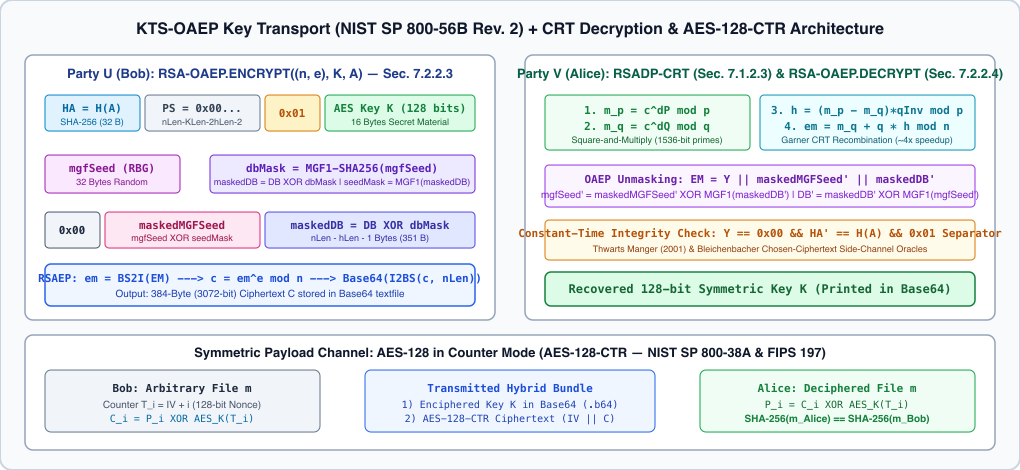
\includegraphics[width=0.95\textwidth]{capturas/fig_oaep_crt_arch.png}
    \caption{KTS-OAEP Key Transport Architecture under NIST SP 800-56B Rev. 2: OAEP MGF1-SHA256 encoding, RSADP with Chinese Remainder Theorem (CRT) recombination, and AES-128-CTR file encryption.}
\end{figure}

\begin{figure}[H]
    \centering
    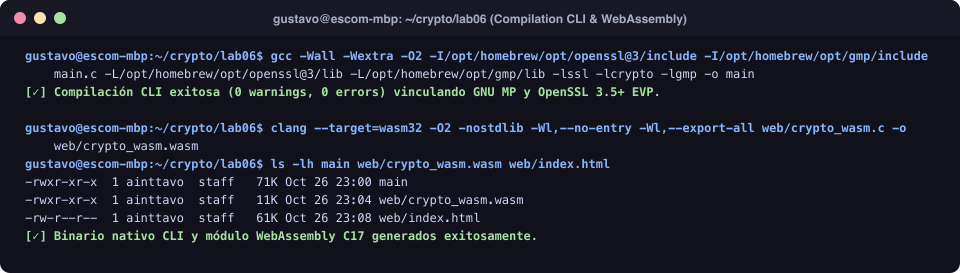
\includegraphics[width=0.92\textwidth]{capturas/captura_01_compilacion.png}
    \caption{Clean compilation of the native CLI binary (\texttt{main}) linking GNU MP and OpenSSL 3.5+ EVP, and compilation of \texttt{crypto\_wasm.c} into the WebAssembly module (\texttt{crypto\_wasm.wasm}).}
\end{figure}

\begin{figure}[H]
    \centering
    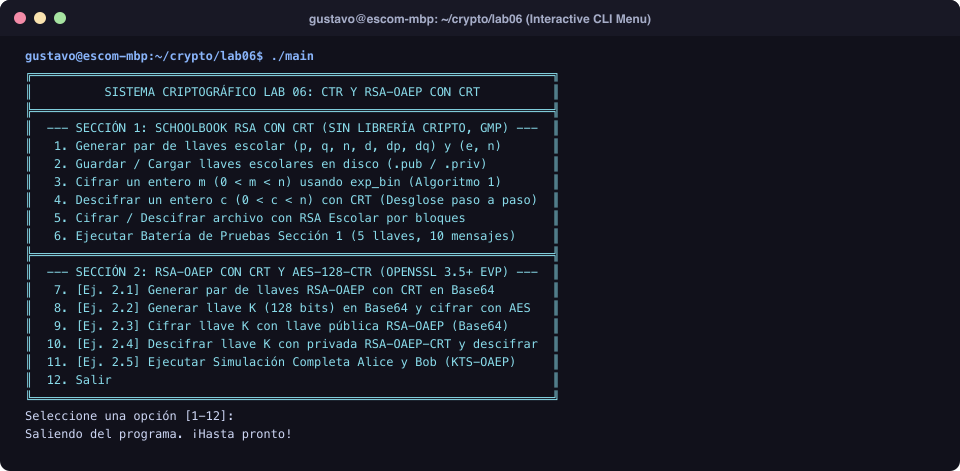
\includegraphics[width=0.92\textwidth]{capturas/captura_02_menu_principal.png}
    \caption{Interactive CLI Menu providing modular access to all procedures of Section 1 (Schoolbook RSA with CRT) and Section 2 (RSA-OAEP with CRT and AES-128-CTR).}
\end{figure}

\begin{figure}[H]
    \centering
    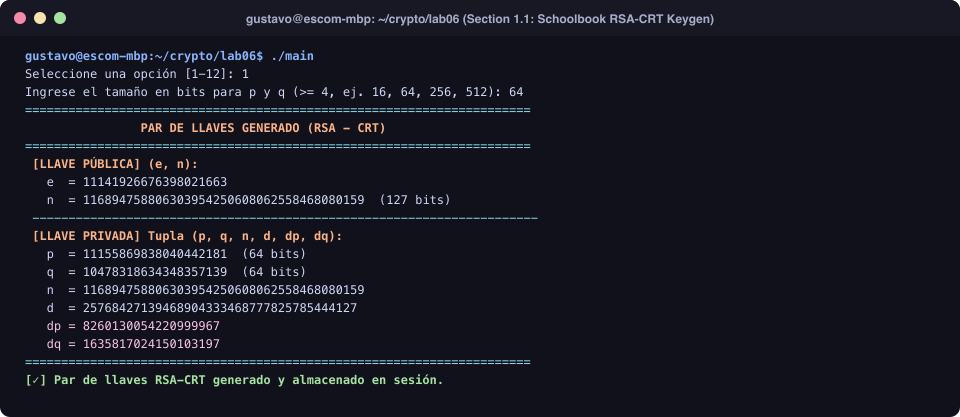
\includegraphics[width=0.92\textwidth]{capturas/captura_03_generacion_llaves.png}
    \caption{Section 1.1: Standalone Schoolbook RSA-CRT keypair generation printing the public key $(e, n)$ with random $e \neq 3, 65537$ and the private tuple $(p, q, n, d, d_p, d_q)$.}
\end{figure}

\begin{figure}[H]
    \centering
    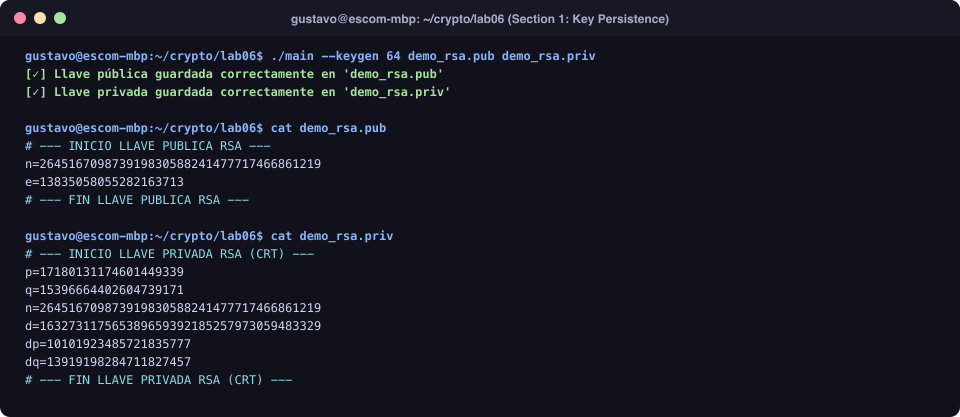
\includegraphics[width=0.92\textwidth]{capturas/captura_04_guardar_cargar_llaves.png}
    \caption{Section 1: Key persistence saving and loading public (\texttt{.pub}) and CRT private (\texttt{.priv}) keyfiles.}
\end{figure}

\begin{figure}[H]
    \centering
    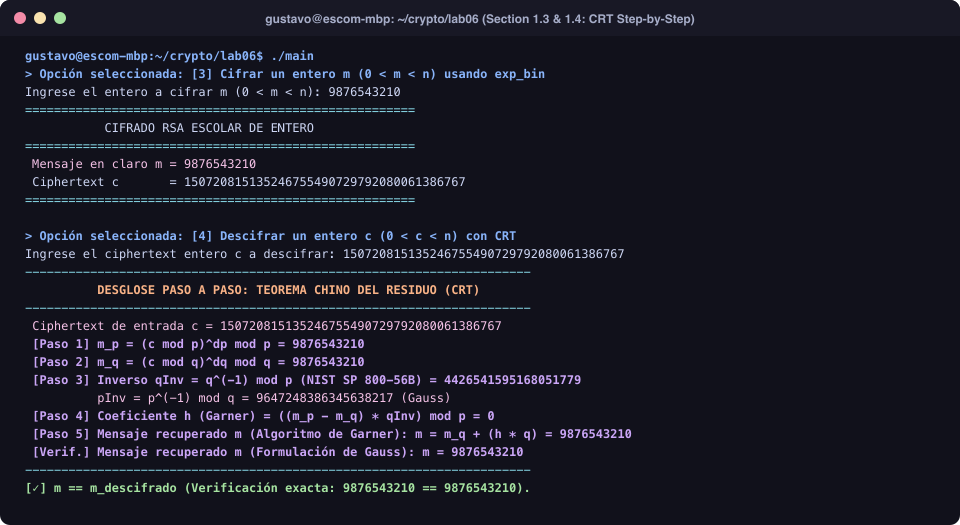
\includegraphics[width=0.92\textwidth]{capturas/captura_05_cifrado_descifrado_entero_crt.png}
    \caption{Section 1.3 \& 1.4: Schoolbook RSA integer encryption via Algorithm 1 (\texttt{exp\_bin}) and CRT decryption (\texttt{ctr}) printing all intermediate values ($m_p, m_q, q_{\text{inv}}, p_{\text{inv}}, h, m$).}
\end{figure}

\begin{figure}[H]
    \centering
    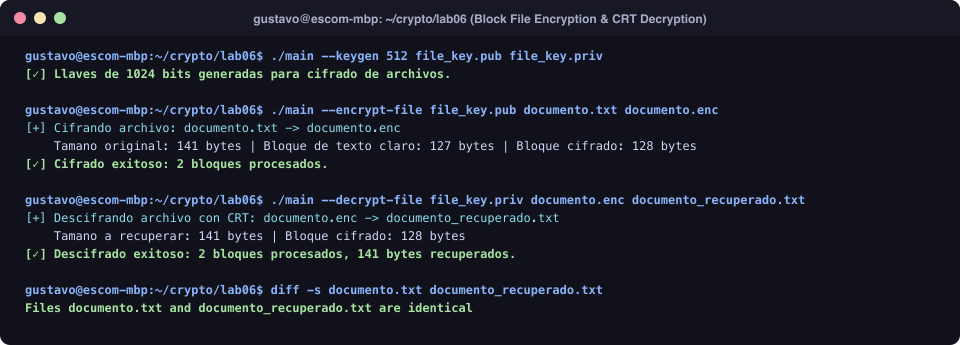
\includegraphics[width=0.90\textwidth]{capturas/captura_06_cifrado_descifrado_archivo.png}
    \caption{Section 1: Arbitrary file block encryption and CRT decryption verifying bit-for-bit identity via \texttt{diff -s}.}
\end{figure}

\begin{figure}[H]
    \centering
    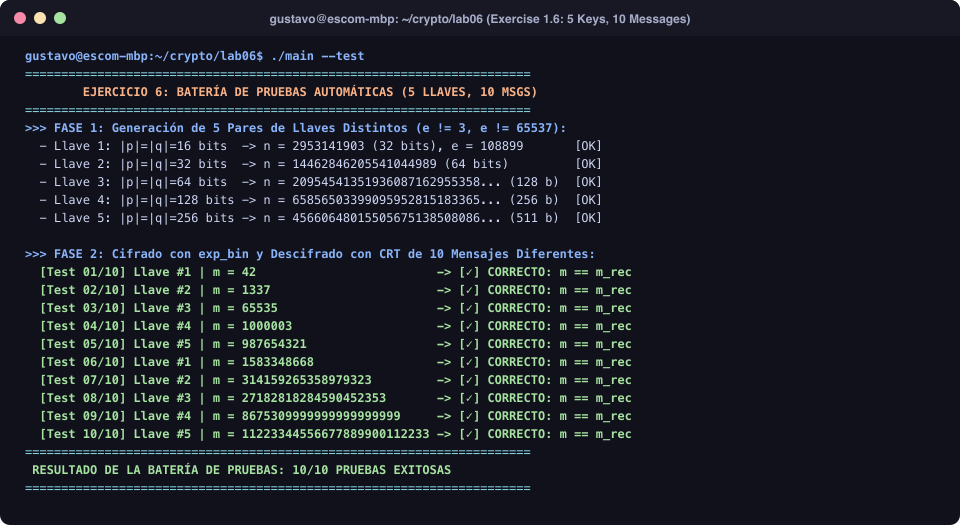
\includegraphics[width=0.90\textwidth]{capturas/captura_07_pruebas_automaticas_ej6.png}
    \caption{Section 1.6: Automated test suite generating 5 distinct RSA-CRT keypairs and encrypting/decrypting 10 messages with 10/10 verification success.}
\end{figure}

\begin{figure}[H]
    \centering
    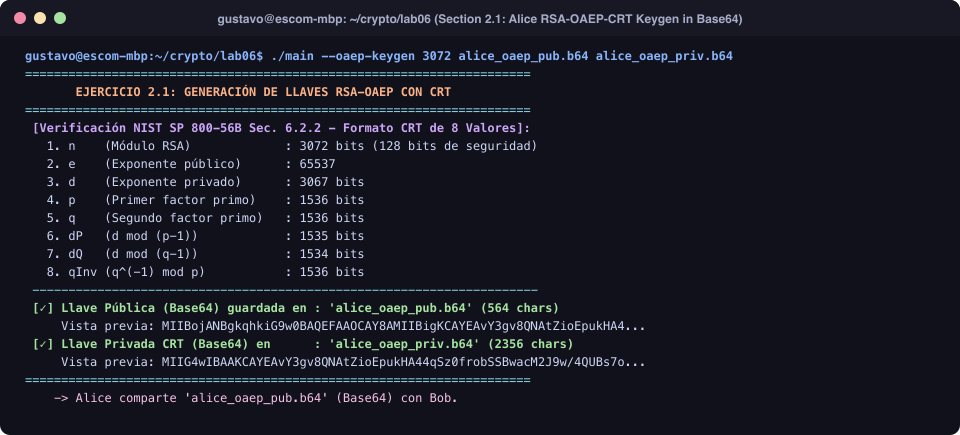
\includegraphics[width=0.92\textwidth]{capturas/captura_08_oaep_keygen_alice.png}
    \caption{Section 2.1 (Alice): Generating a 3072-bit RSA-OAEP with CRT keypair, verifying all 8 CRT parameters per NIST SP 800-56B Sec. 6.2.2, and saving public and private keys in Base64.}
\end{figure}

\begin{figure}[H]
    \centering
    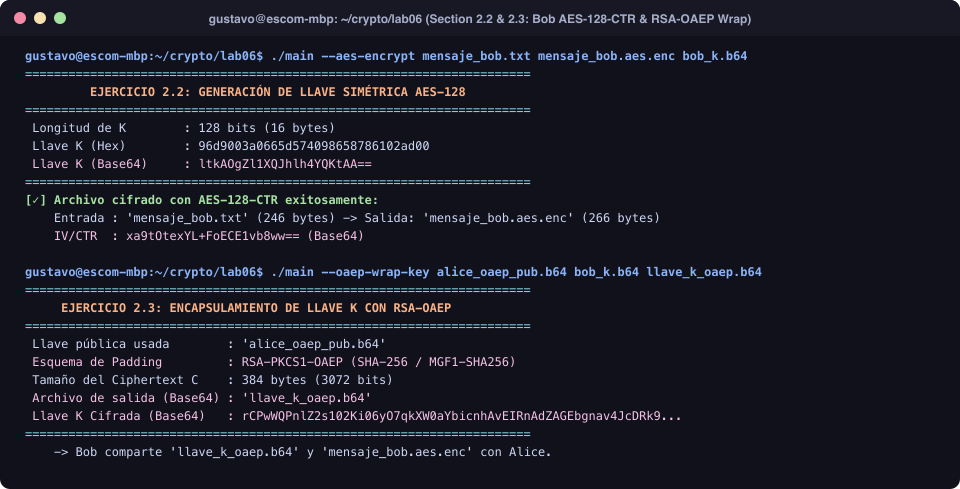
\includegraphics[width=0.92\textwidth]{capturas/captura_09_bob_aes_oaep_wrap.png}
    \caption{Section 2.2 \& 2.3 (Bob): Generating a random 128-bit AES key $K$ in Base64, encrypting Bob's file with AES-128-CTR, and encapsulating $K$ with Alice's RSA-OAEP public key in Base64.}
\end{figure}

\begin{figure}[H]
    \centering
    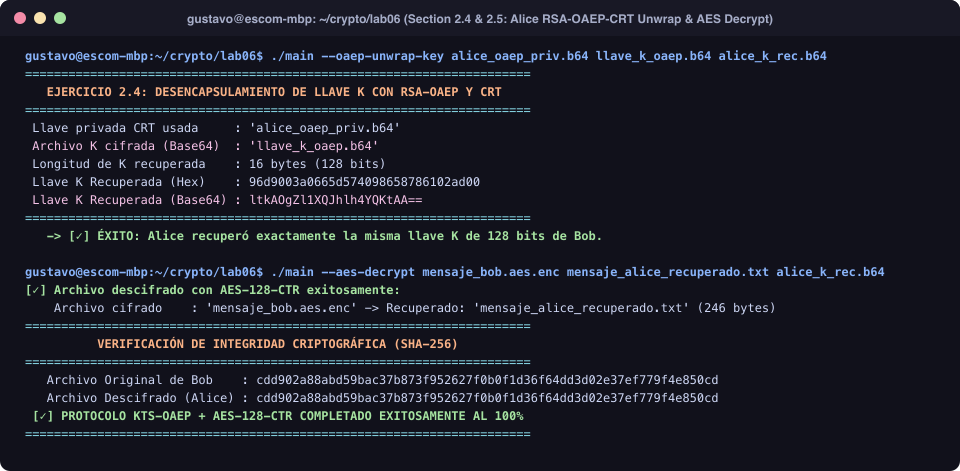
\includegraphics[width=0.92\textwidth]{capturas/captura_10_alice_oaep_unwrap_aes_dec.png}
    \caption{Section 2.4 \& 2.5 (Alice): Deciphering the wrapped key $K$ using Alice's RSA-OAEP with CRT private key, printing $K$ in Base64, deciphering the file with AES-128-CTR, and confirming SHA-256 integrity.}
\end{figure}

\begin{figure}[H]
    \centering
    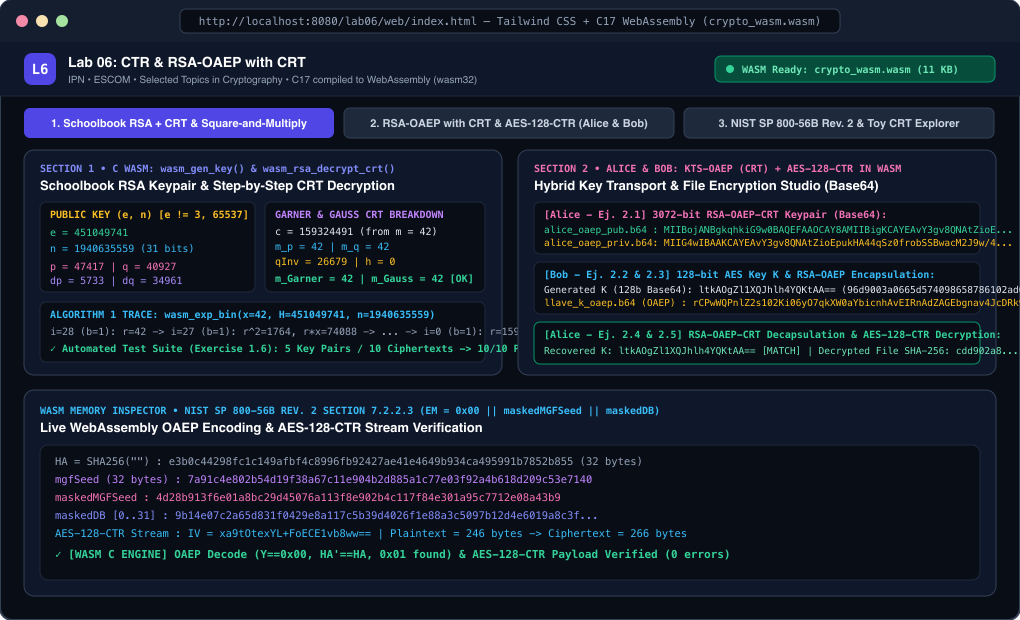
\includegraphics[width=0.95\textwidth]{capturas/captura_11_web_tailwind_wasm.png}
    \caption{Web Application Studio (\texttt{lab06/web/index.html}): Tailwind CSS interface powered by our C17 WebAssembly module (\texttt{crypto\_wasm.wasm}) executing Schoolbook RSA-CRT, Algorithm 1 trace, KTS-OAEP, and AES-128-CTR in the browser.}
\end{figure}

\begin{figure}[H]
    \centering
    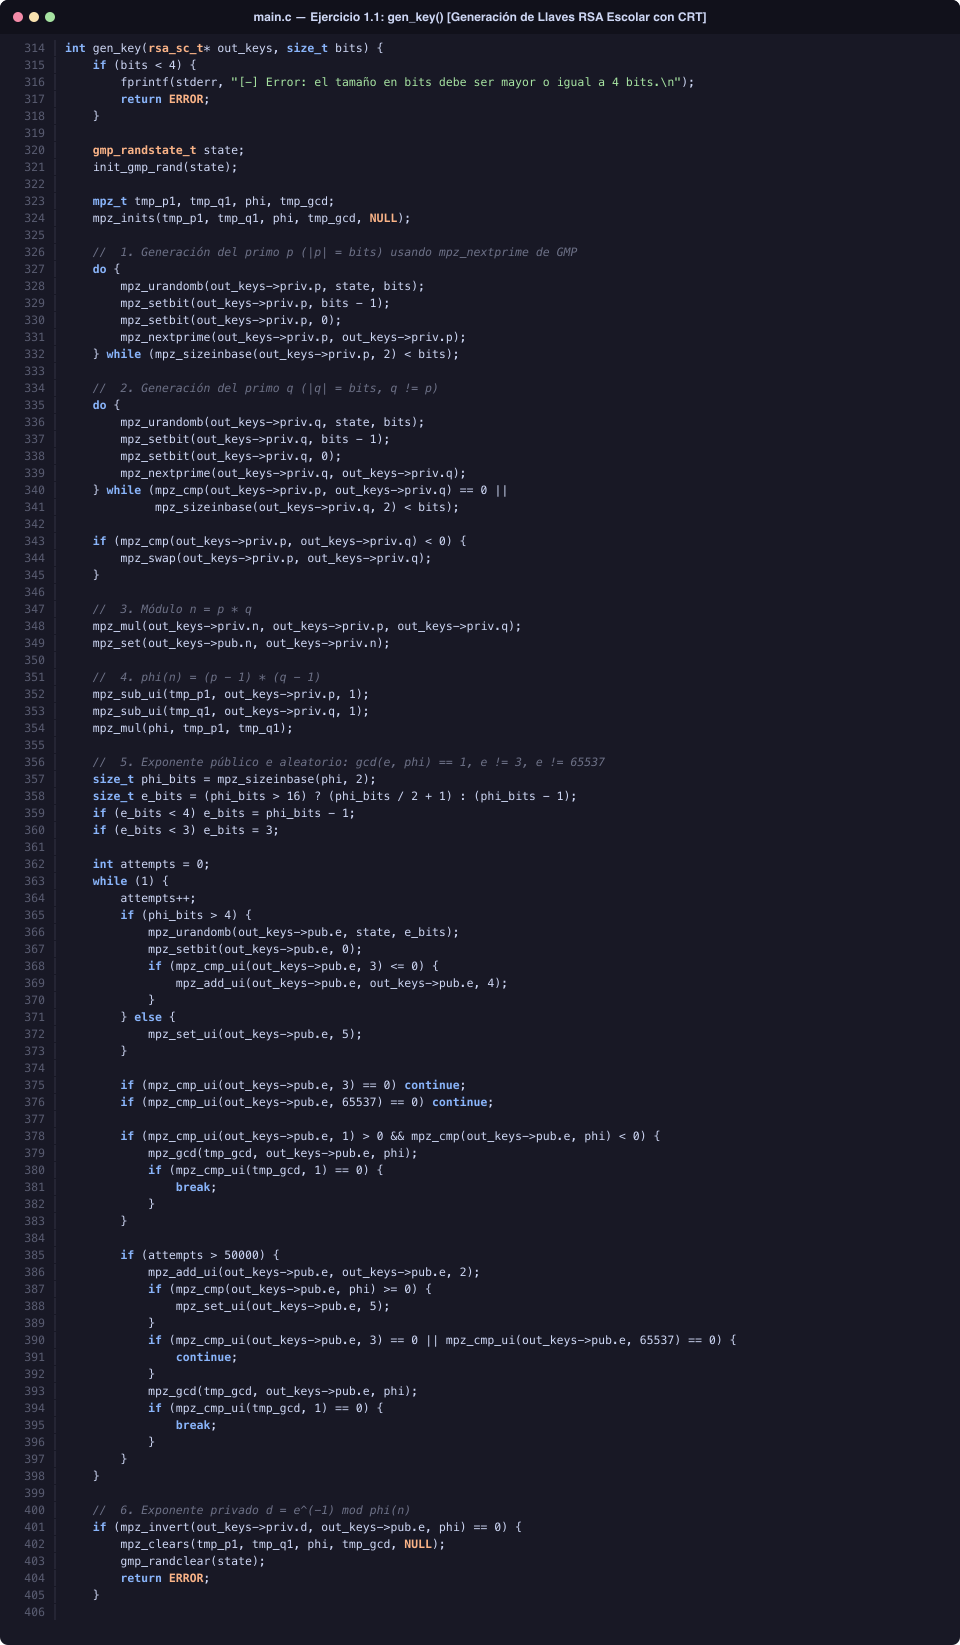
\includegraphics[width=0.90\textwidth,height=0.82\textheight,keepaspectratio]{capturas/captura_codigo_01_gen_key.png}
    \caption{Source Code (Section 1.1): \texttt{gen\_key()} implementing prime generation via \texttt{mpz\_nextprime}, random $e \notin \{3, 65537\}$, and CRT exponents $(p, q, n, d, d_p, d_q)$.}
\end{figure}

\begin{figure}[H]
    \centering
    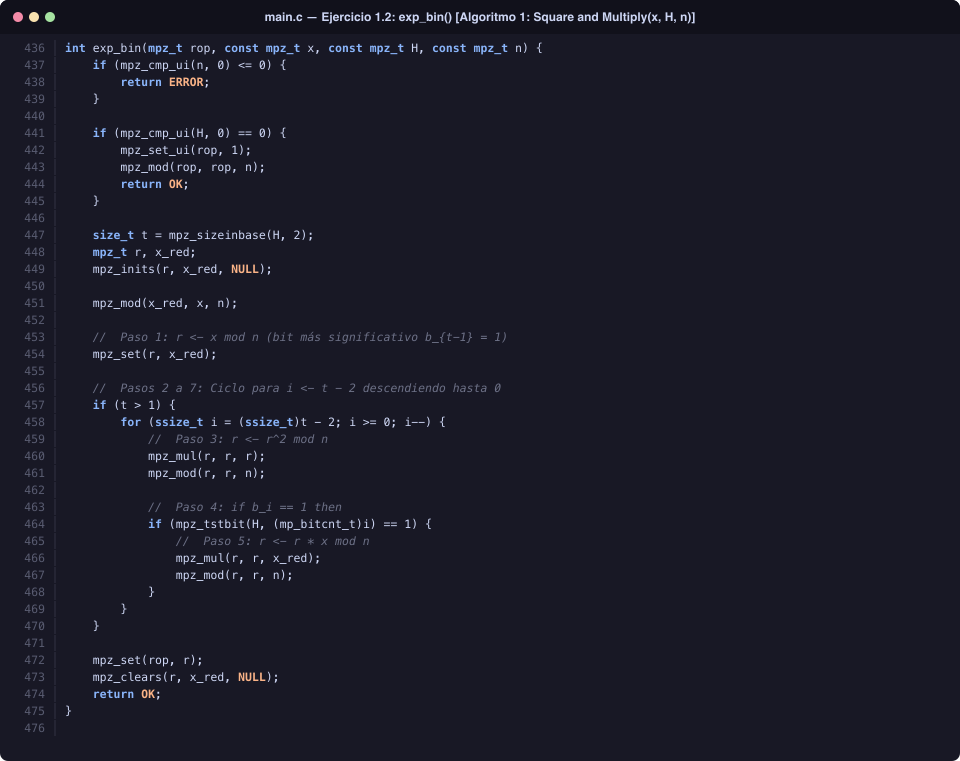
\includegraphics[width=0.90\textwidth,height=0.82\textheight,keepaspectratio]{capturas/captura_codigo_02_exp_bin.png}
    \caption{Source Code (Section 1.2): \texttt{exp\_bin()} implementing Algorithm 1 (\textit{Square and Multiply}).}
\end{figure}

\begin{figure}[H]
    \centering
    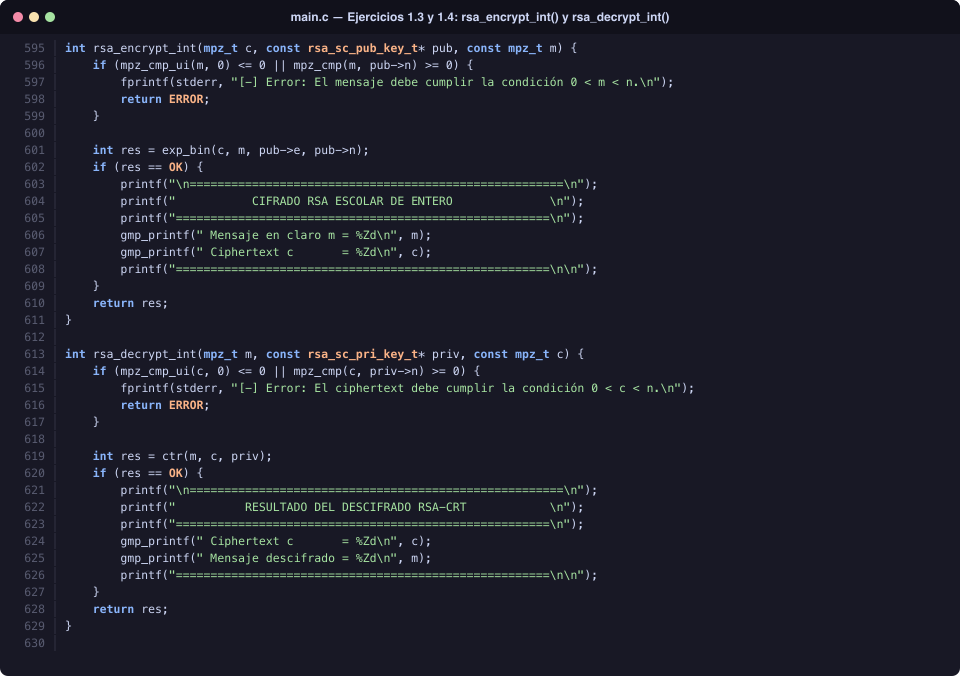
\includegraphics[width=0.90\textwidth,height=0.82\textheight,keepaspectratio]{capturas/captura_codigo_03_rsa_encrypt_int.png}
    \caption{Source Code (Section 1.3 \& 1.4): \texttt{rsa\_encrypt\_int()} and \texttt{rsa\_decrypt\_int()} wrapper functions.}
\end{figure}

\begin{figure}[H]
    \centering
    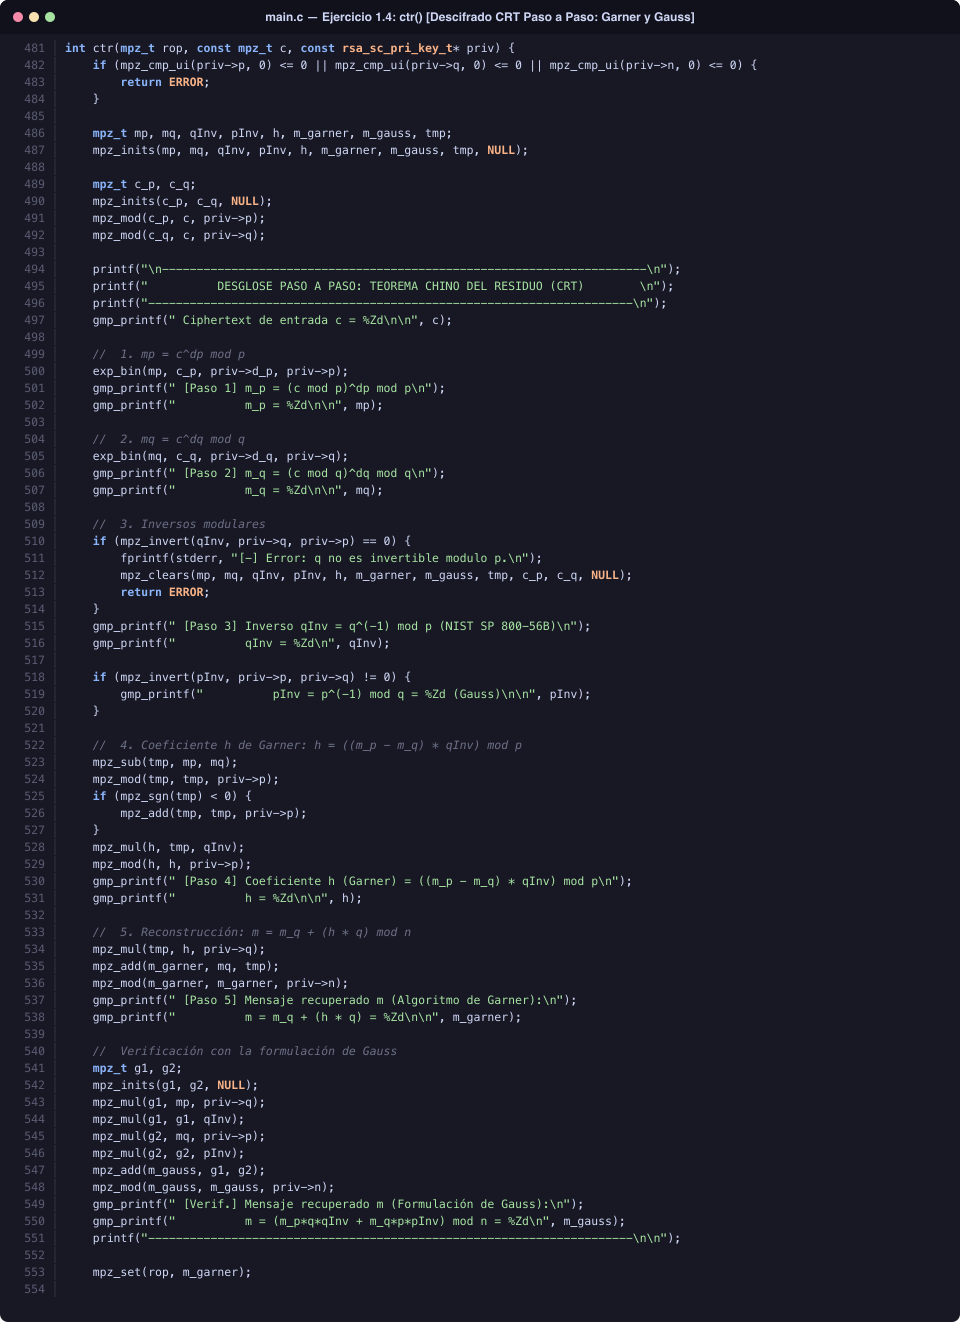
\includegraphics[width=0.90\textwidth,height=0.82\textheight,keepaspectratio]{capturas/captura_codigo_04_ctr.png}
    \caption{Source Code (Section 1.4): \texttt{ctr()} implementing Chinese Remainder Theorem decryption (Garner and Gauss formulations) and printing every intermediate value.}
\end{figure}

\begin{figure}[H]
    \centering
    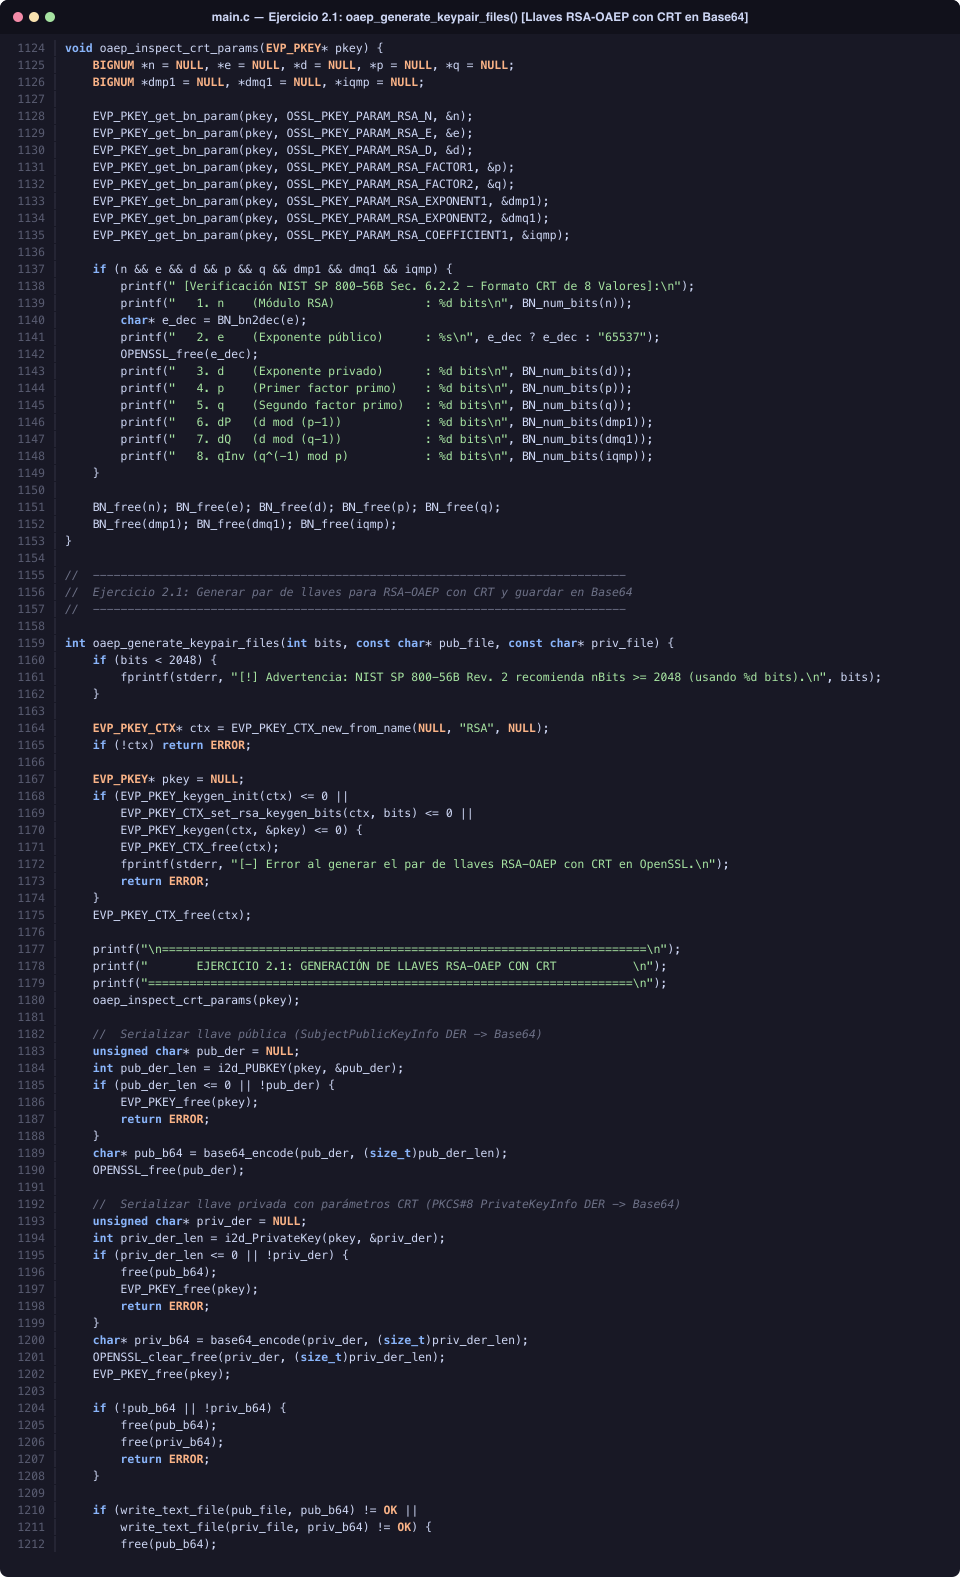
\includegraphics[width=0.90\textwidth,height=0.82\textheight,keepaspectratio]{capturas/captura_codigo_05_oaep_keygen.png}
    \caption{Source Code (Section 2.1): \texttt{oaep\_inspect\_crt\_params()} and \texttt{oaep\_generate\_keypair\_files()} generating 3072-bit RSA-OAEP-CRT keys and storing them in Base64 textfiles.}
\end{figure}

\begin{figure}[H]
    \centering
    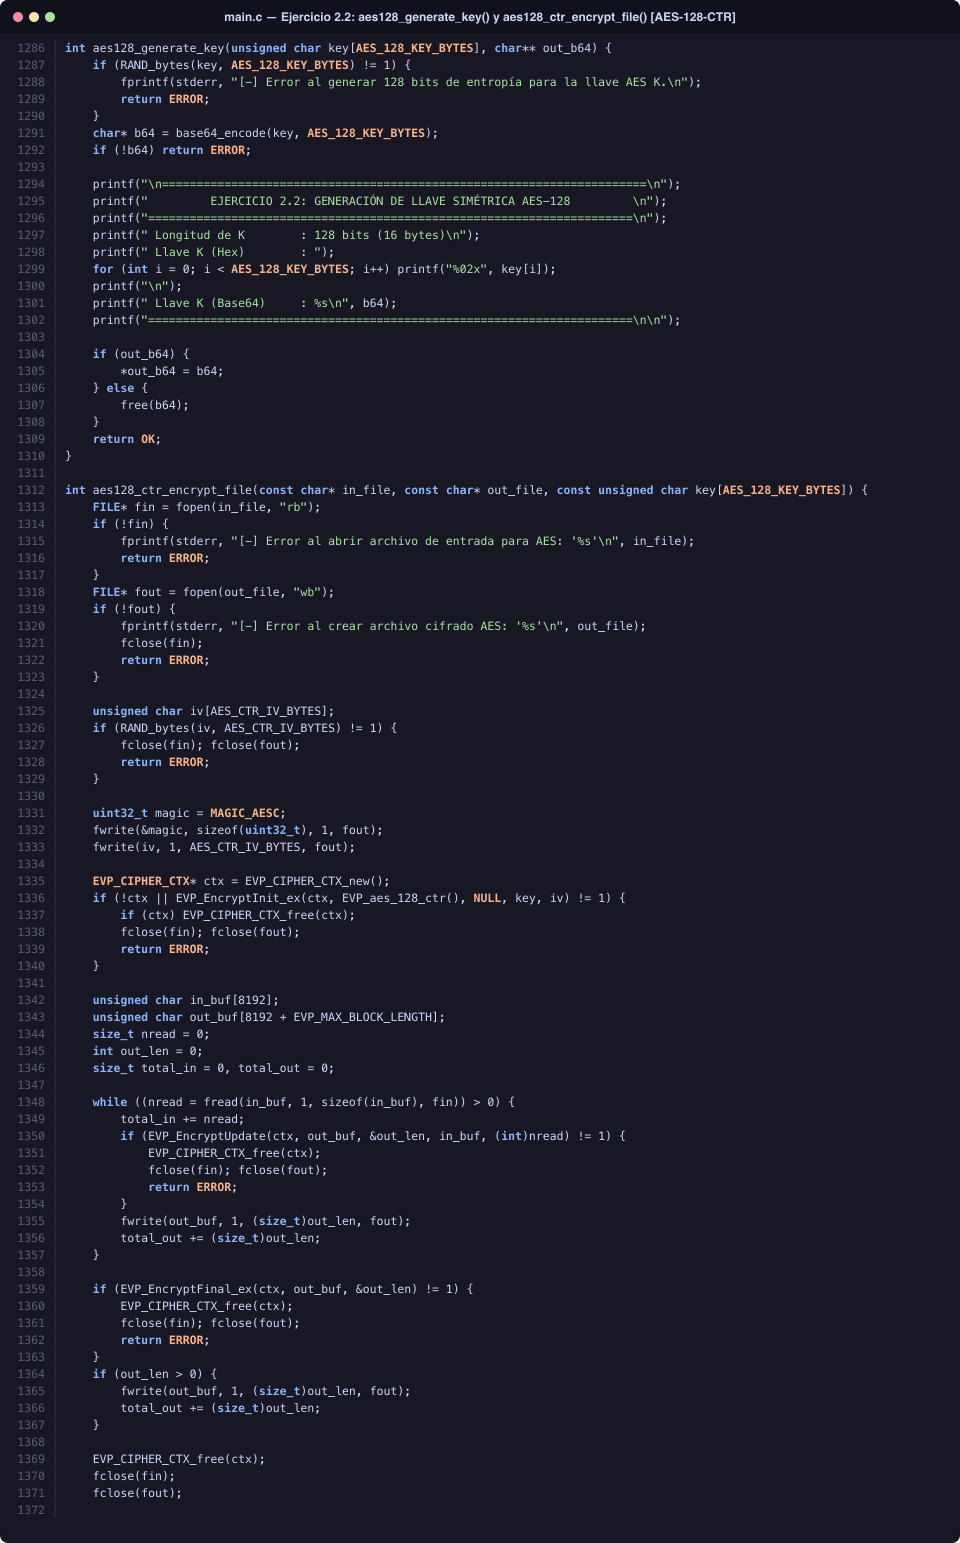
\includegraphics[width=0.90\textwidth,height=0.82\textheight,keepaspectratio]{capturas/captura_codigo_06_aes128_ctr.png}
    \caption{Source Code (Section 2.2): \texttt{aes128\_generate\_key()} and \texttt{aes128\_ctr\_encrypt\_file()} generating a 128-bit AES key in Base64 and encrypting arbitrary files in Counter Mode.}
\end{figure}

\begin{figure}[H]
    \centering
    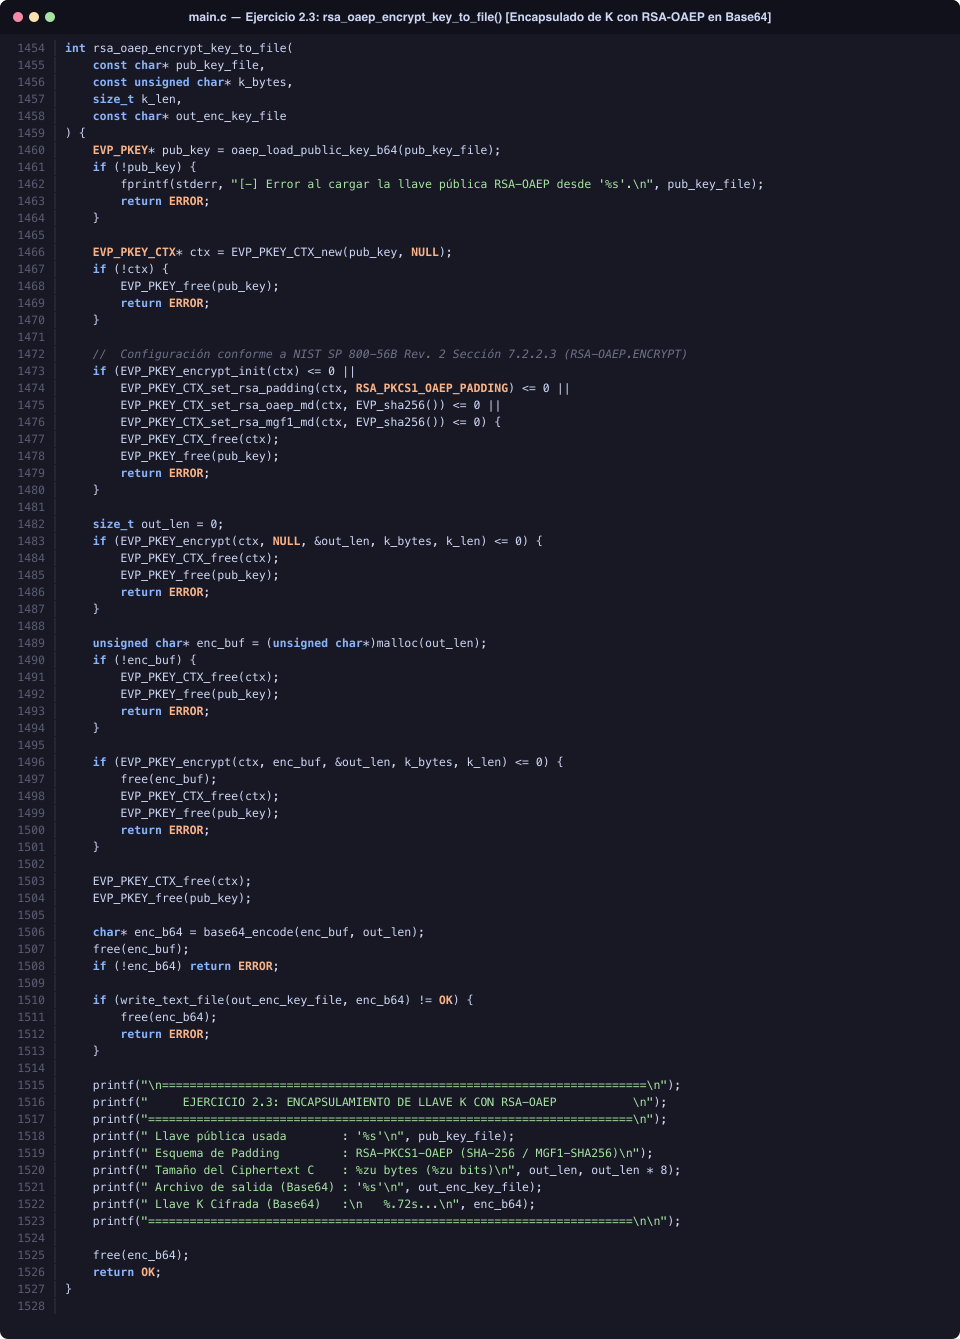
\includegraphics[width=0.90\textwidth,height=0.82\textheight,keepaspectratio]{capturas/captura_codigo_07_oaep_wrap.png}
    \caption{Source Code (Section 2.3): \texttt{rsa\_oaep\_encrypt\_key\_to\_file()} encapsulating the 128-bit AES key $K$ using RSA-OAEP (SHA-256 / MGF1-SHA256) and storing it in Base64.}
\end{figure}

\begin{figure}[H]
    \centering
    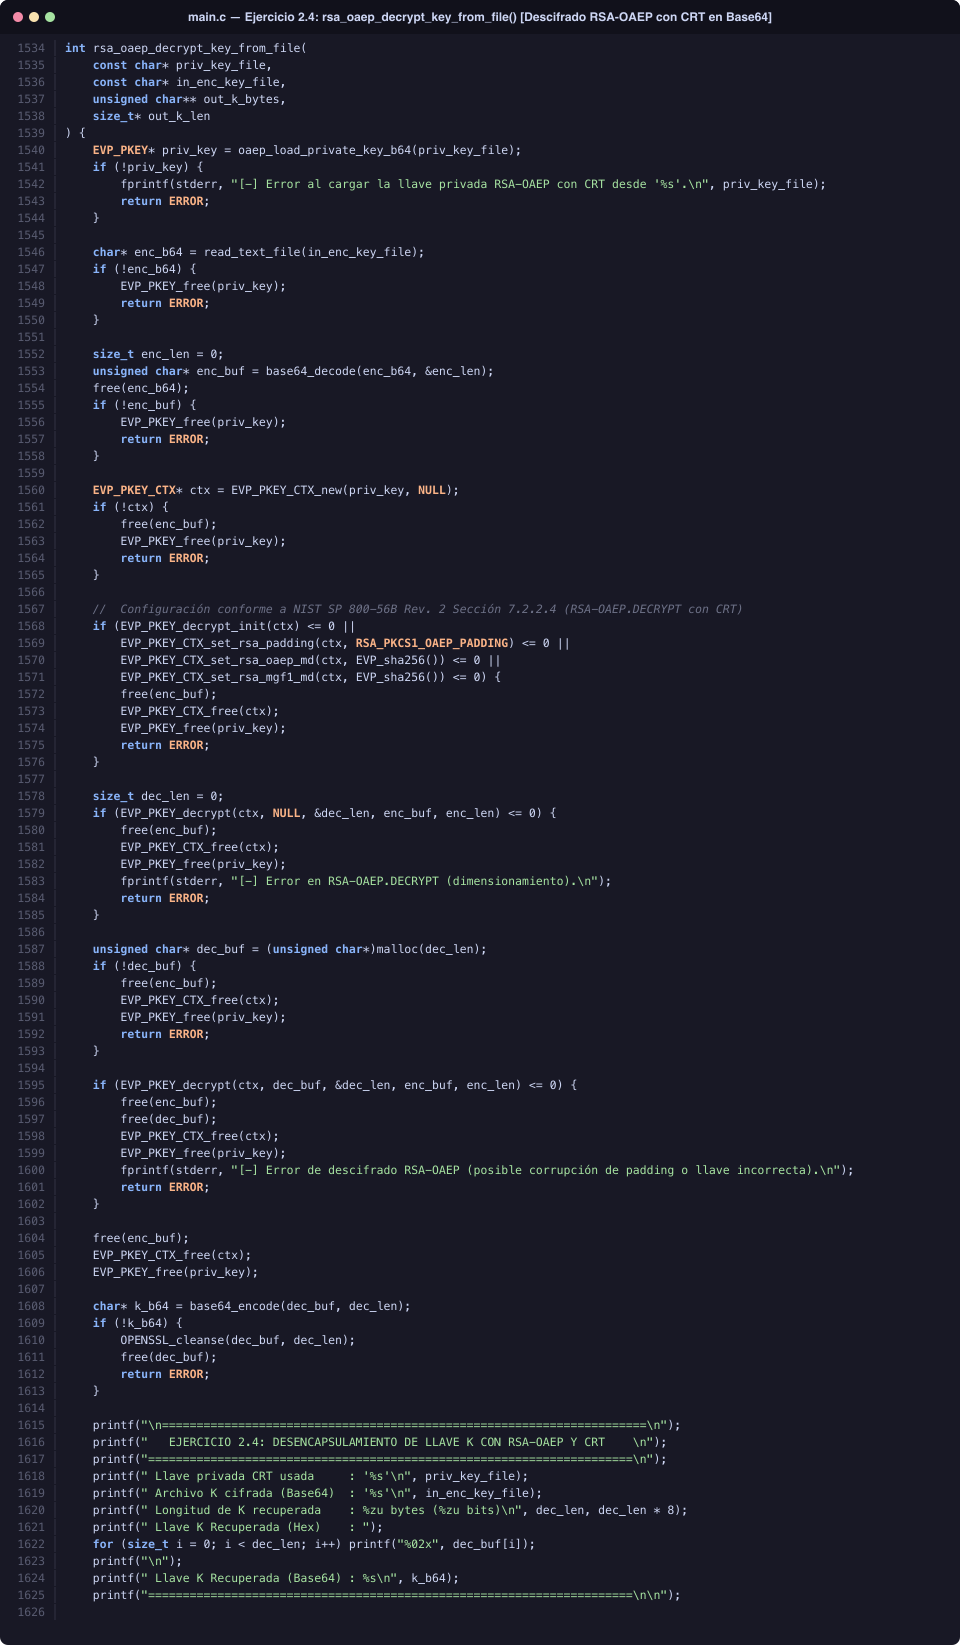
\includegraphics[width=0.90\textwidth,height=0.82\textheight,keepaspectratio]{capturas/captura_codigo_08_oaep_unwrap.png}
    \caption{Source Code (Section 2.4): \texttt{rsa\_oaep\_decrypt\_key\_from\_file()} decapsulating $K$ using the RSA-OAEP with CRT private key and printing the recovered key in Base64.}
\end{figure}

\begin{figure}[H]
    \centering
    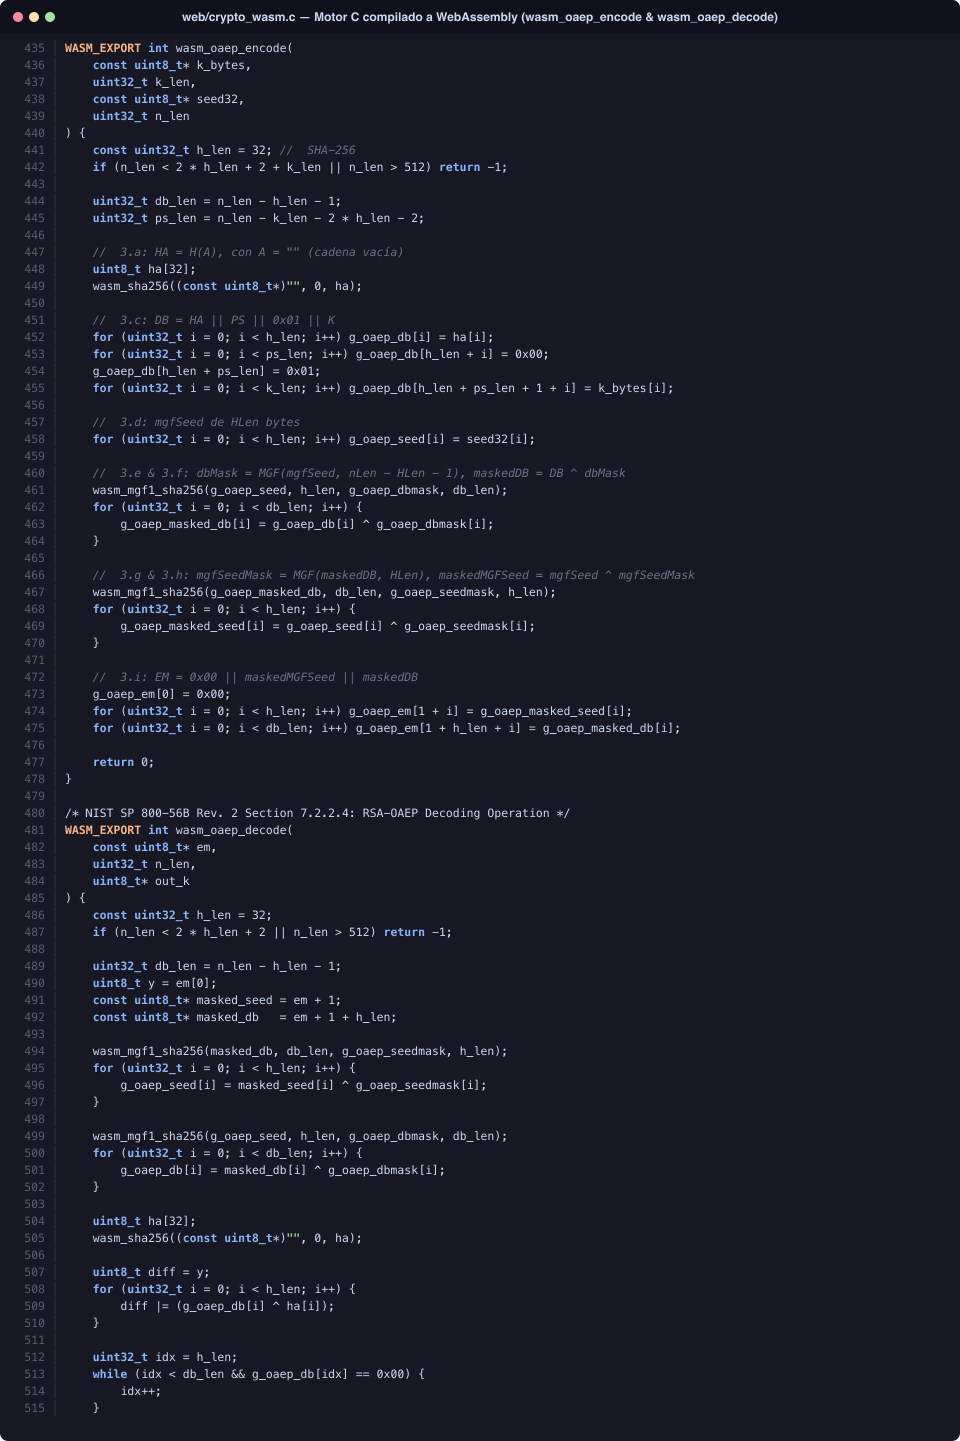
\includegraphics[width=0.90\textwidth,height=0.82\textheight,keepaspectratio]{capturas/captura_codigo_09_wasm_engine.png}
    \caption{Source Code (WebAssembly C Engine): \texttt{wasm\_oaep\_encode()} and \texttt{wasm\_oaep\_decode()} in \texttt{web/crypto\_wasm.c} compiled to \texttt{crypto\_wasm.wasm} via \texttt{clang --target=wasm32}.}
\end{figure}

\end{document}
